\input{/Users/daniel/Documents/LaTeX/article-style.tex}

\hypersetup{
  pdfauthor = {Daniel Schreurs},
  pdftitle = {Développement d'applications mobiles : Projet d'examen},
  pdfsubject = {Développement d'applications mobiles},
  pdfkeywords = {Enoncé, DAM, Flutter, 3e, INPRES},
  pdfcreator = {LuaLaTeX},
  pdfproducer = {LuaLaTeX},
  breaklinks  = true,
  colorlinks  = true,
  allcolors   = blue
  % hidelinks   = true,
  % linkcolor   = blue,
  % anchorcolor = red,
  % citecolor   = blue,
  % filecolor   = red,
  % urlcolor    = blue
}

%%%%%%%%%%%%%%%%%%%%%%%%%%%%%%%%%%%%%%%%%%%%%%%%%%%%%%%%%%%
% CONFIGURATION OF LISTING PACKAGE
%%%%%%%%%%%%%%%%%%%%%%%%%%%%%%%%%%%%%%%%%%%%%%%%%%%%%%%%%%%

\lstset{basicstyle=\ttfamily,tabsize=2,mathescape=true,commentstyle=\itshape}
\lstdefinestyle{inline}{extendedchars=true,breaklines=true,basicstyle=\ttfamily,mathescape=false}
\lstdefinestyle{code}{extendedchars=true,tabsize=2,breaklines=true,mathescape=false}
\lstdefinestyle{examples}{extendedchars=true,tabsize=2,breaklines=true,basicstyle=\ttfamily\small,mathescape=false}
\lstdefinestyle{command}{extendedchars=true,tabsize=2,breaklines=true,basicstyle=\ttfamily,mathescape=false,moredelim=[is][\itshape]{!}{!},moredelim=[is][\bfseries]{?}{?},escapeinside={}}
\lstMakeShortInline[extendedchars=true,breaklines=true,basicstyle=\ttfamily]£
\lstdefinestyle{exampleblk}{xleftmargin=0pt, linewidth=\textwidth, extendedchars=true, tabsize=2, breaklines=true, breakindent=0pt, prebreak=\raisebox{0ex}[0ex][0ex]{\ensuremath{\hookleftarrow}}, basicstyle=\ttfamily, mathescape=false, numbers=none, moredelim=[is][\bfseries\underbar]{ß}{ß}, moredelim=[is][\bfseries]{£}{£}, frame=single}

%%%%%%%%%%%%%%%%%%%%%%%%%%%%%%%%%%%%%%%%%%%%%%%%%%%%%%%%%%%
% HEADER AND FOOTER
%%%%%%%%%%%%%%%%%%%%%%%%%%%%%%%%%%%%%%%%%%%%%%%%%%%%%%%%%%%

\newpagestyle{mypagestyle}{%
\sethead{HEPL}{MMI}{D. Schreurs}
\setfoot{}{}{Page \thepage \hspace{1pt} sur \pageref*{LastPage}}
\headrule
}


%%%%%%%%%%%%%%%%%%%%%%%%%%%%%%%%%%%%%%%%%%%%%%%%%%%%%%%%%%%
% SECTION HEADINGS (TITLESEC PACKAGE)
%%%%%%%%%%%%%%%%%%%%%%%%%%%%%%%%%%%%%%%%%%%%%%%%%%%%%%%%%%%
\makeatletter

\makeatother

\def\emaildaniel{\href{mailto:daniel.schreurs@hepl.be}{daniel.schreurs@hepl.be}}
\title{Projet d'évaluation continue\\[3mm]AA : MMI - Multimédia Intéractif - TP\\[3mm]\large 2\textsuperscript{e} Bachelier en techniques graphiques, orientation techniques infographiques option Web\\Haute École de la Province de Liège (HEPL)}
\author{Daniel Schreurs \textless\emaildaniel\textgreater}
\date{2021 -- 2022}


\begin{document}

\pagestyle{mypagestyle}

\maketitle

%%%%%%%%%%%%%%%%%%%%%%%%%%%%%%%%%%%%%%%%%%%%%%%%%%%%%%%%%%%
% SECTION
%%%%%%%%%%%%%%%%%%%%%%%%%%%%%%%%%%%%%%%%%%%%%%%%%%%%%%%%
\section{Introduction}

L’objectif de ce travail est de vous donner une occasion supplémentaire pour entrainer votre maitrise de JavaScript, votre connaissance de l'API Canvas ainsi que la structure type d'un projet, tel que vue en classe. L'idée étant de reproduire le plus fidèlement possible un jeu populaire. Vous pouvez vous intéresser \href{https://archive.org/details/internetarcade}{aux jeux d'arcades}, par exemple.

\subsection{Procédure}
\label{procedure}

\begin{itemize}
  \item Rendez-vous sur \href{https://classroom.github.com/a/xBzM63w9}{cette page}.
  \item Acceptez le devoir. Ensuite, vous serez redirigés vers une page qui contient le lien de votre dépôt\footnote{Il est nécessaire de rafraichir la page pour voir ce lien apparaitre.}.
  \item Rendez-vous dans les réglages de votre dépôt afin de renommer celui-ci. Le but étant de remplacer votre nom d'utilisateur par votre nom suivi de votre prénom. Le nom de votre dépôt doit nécessairement devenir \verb!projet-mmi-juin-linus-torvalds!. En remplaçant \verb!torvalds! par votre nom et \verb!linus! par votre prénom~\footnote{Notez qu’il n'y a pas d'espaces et de majuscules. Seuls les tirets séparent les mots. Suivez la notation \href{https://en.wiktionary.org/wiki/kebab_case}{kebab-case}.}.
  \item Dès lors que vous avez renommé votre dépôt, vous pouvez le cloner et commencer la rédaction du document \verb!readme.md!.
\end{itemize}
\vspace*{2cm}
\begin{figure}[htbp]
  \centering
  \includesvg{img/gost.svg}
\end{figure}

\clearpage
\section{Contenu du dépôt}
\label{La documentation}

Votre dépôt doit au moins contenir :
\begin{itemize}
  \item Un document \verb!readme.md! avec :
        \begin{itemize}
          \item Une présentation du jeu que vous souhaitez reproduire. Donc qui l'a inventé, son contexte, langage, etc.
          \item Si vous créez votre propre jeu, vous devez fournir une petite étude de l'existant. Quels sont les jeux qui y ressemblent~avec éventuellement un avis.
          \item Détailler les règles du jeu.
          \item Fournir la liste des règles que vous allez reprendre et/ou adapter.
          \item Fournir une liste des points qu'il reste à faire ou qui méritent d'être améliorés. Cette liste doit-être maintenant au début, pendant et surtout à la fin de votre projet. Elle permet d'acter votre état d'avancement un peu comme une todolist.\footnote{Notez qu'il est donc très intéressant de se servir des \href{https://stackoverflow.com/questions/47344571/how-to-draw-checkbox-or-tick-mark-in-github-markdown-table}{cases à cocher}.}
        \end{itemize}
  \item Si vous êtes amené à redessiner certaines illustrations, vous devez fournir les sources. Notez que certaines ressources sont disponibles sur \href{https://www.spriters-resource.com}{spriters-resource.com}.
  \item Vous devez également mettre à jour les \href{https://realfavicongenerator.net}{favicons}.
\end{itemize}

\section{Évaluation}

Ce projet constitue l'une des 2 cotes de l'évaluation continue. En plus de fournir une expérience utilisateur aboutie, votre jeu doit nécessairement respecter l'ensemble des \href{https://github.com/hepl-dcc/dcc-guidelines}{bonnes pratiques JavaScript} et \href{https://github.com/hepl-mmi/mmi-guidelines}{TypeScript}.
Ce projet sera clôturé, la veille du jour de l'examen. Vous devez publier votre jeu grâce aux \href{https://docs.github.com/en/pages/getting-started-with-github-pages/configuring-a-publishing-source-for-your-github-pages-site}{GitHub Pages}. Il s'agit simplement d'une option à activer dans les réglages de votre projet, comme illustré dans la capture ci-dessous.

\vspace*{1cm}

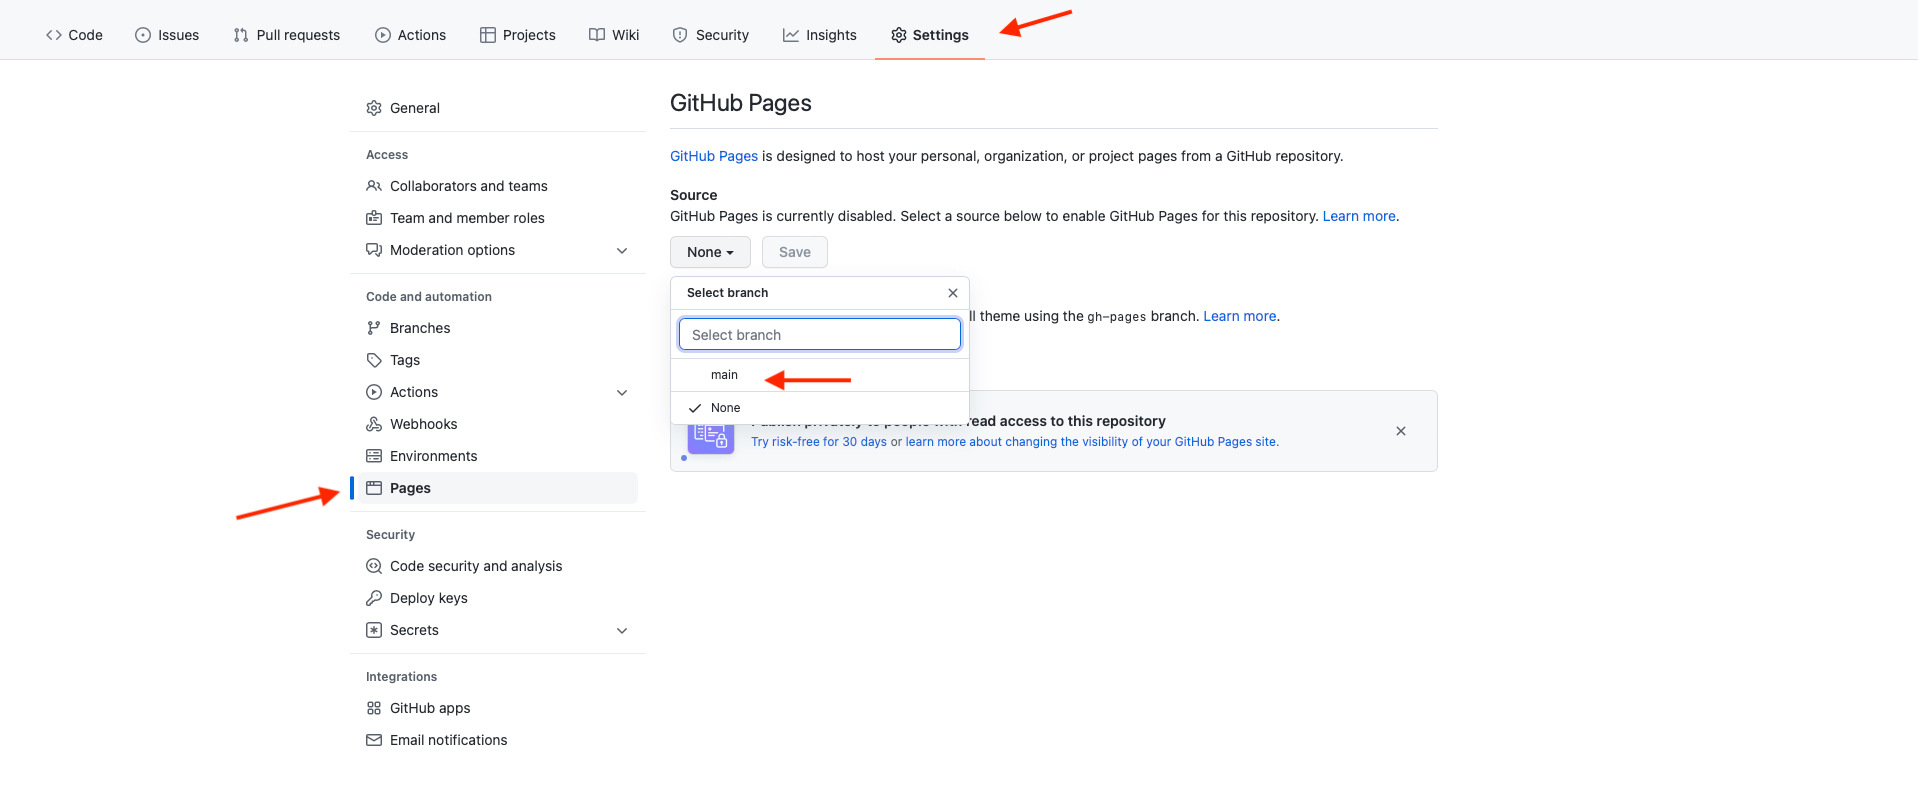
\includegraphics[width=\textwidth]{img/pages.jpg}

\end{document}
